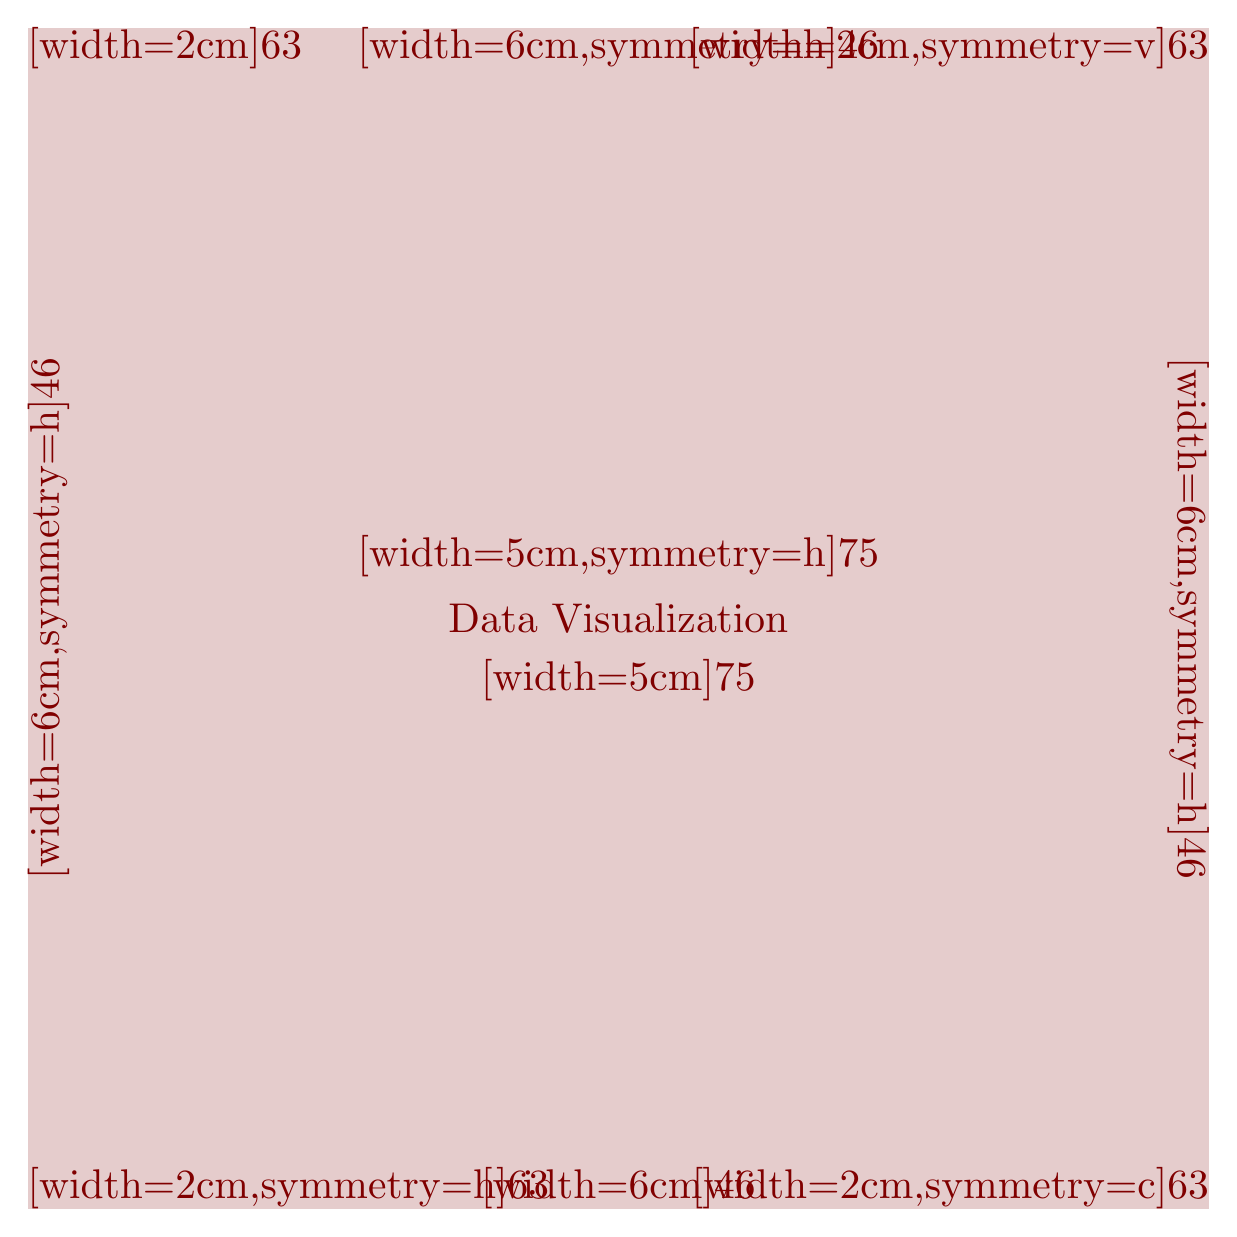
\begin{tikzpicture}[color=Maroon, transform shape, scale=1.5,
        every node/.style={inner sep=0pt}]
    % Background box
    \node[minimum size=10cm, fill=Maroon!20, inner sep=0pt](vecbox){};
    
    % Corner ornaments
    \node[anchor=north west] at (vecbox.north west){\pgfornament[width=2cm]{63}};
    \node[anchor=north east] at (vecbox.north east){\pgfornament[width=2cm,symmetry=v]{63}};
    \node[anchor=south west] at (vecbox.south west){\pgfornament[width=2cm,symmetry=h]{63}};
    \node[anchor=south east] at (vecbox.south east){\pgfornament[width=2cm,symmetry=c]{63}};
    
    % Side ornaments
    \node[anchor=north] at (vecbox.north){\pgfornament[width=6cm,symmetry=h]{46}};
    \node[anchor=south] at (vecbox.south){\pgfornament[width=6cm]{46}};
    \node[anchor=north, rotate=90] at (vecbox.west){\pgfornament[width=6cm,symmetry=h]{46}};
    \node[anchor=north, rotate=-90] at (vecbox.east){\pgfornament[width=6cm,symmetry=h]{46}};
    
    % Center text
    \node[inner sep=6pt] (text) at (vecbox.center) {Data Visualization};
    
    % Ornaments around the text
    \node[anchor=north] at (text.south) {\pgfornament[width=5cm]{75}};
    \node[anchor=south] at (text.north) {\pgfornament[width=5cm,symmetry=h]{75}};
\end{tikzpicture}
